% Hlavicka pro protokoly z fyzikalniho praktika.
% Verze pro: LaTeX
% Verze hlavicky: 22. 2. 2007
% Autor: Ustav fyziky kondenzovanych latek
% Ke stazeni: www.physics.muni.cz/ufkl/Vyuka/
% Licence: volne k pouziti, nejlepe k vcasnemu odevzdani protokolu z Vaseho mereni.

\documentclass[a4paper,11pt]{article}

% Kodovani (cestiny) v dokumentu: utf-8
%\usepackage[cp1250]{inputenc}	% Omezena stredoevropska kodova stranka, pouze MSW.
\usepackage[utf8]{inputenc}	% Doporucujeme pouzivat UTF-8 (unicode).
\usepackage[T1]{fontenc}
\usepackage{lmodern}

%%% Nemente:
\usepackage[margin=2cm]{geometry}
\newtoks\jmenopraktika \newtoks\jmeno \newtoks\datum
\newtoks\obor \newtoks\skupina \newtoks\rocnik \newtoks\semestr
\newtoks\cisloulohy \newtoks\jmenoulohy
\newtoks\tlak \newtoks\teplota \newtoks\vlhkost
\usepackage{amsmath}
\usepackage{mathtools}
\usepackage{graphicx}
\usepackage{multirow}

\usepackage{pgfplotstable} 
\usepackage{booktabs}

\graphicspath{ {./images/} }
%%% Nemente - konec.


%%%%%%%%%%% Doplnte pozadovane polozky:

\jmenopraktika={Fyzikální praktikum 3}  % nahradte jmenem vaseho predmetu
\jmeno={Artem Gorodilov}            % nahradte jmenem mericiho
\datum={11. ~března 2024}        % nahradte datem mereni ulohy
\obor={Astrofyzika}                     % nahradte zkratkou vami studovaneho oboru
\skupina={Po 14:00}            % nahradte dobou vyuky vasi seminarni skupiny
\rocnik={II}                  % nahradte rocnikem, ve kterem studujete
\semestr={II}                 % nahradte semestrem, ve kterem studujete

\cisloulohy={A}               % nahradte cislem merene ulohy
\jmenoulohy={Pohyb nábojů v elektrickém a magnetickém poli} % nahradte jmenem merene ulohy

\tlak={979}                   % nahradte tlakem pri mereni (v hPa)
\teplota={21.4}               % nahradte teplotou pri mereni (ve stupnich Celsia)
\vlhkost={46}               % nahradte vlhkosti vzduchu pri mereni (v %)

%%%%%%%%%%% Konec pozadovanych polozek.


%%%%%%%%%%% Uzitecne balicky:
\usepackage[czech]{babel}
\usepackage{graphicx}
\usepackage{amsmath}
\usepackage{xspace}
\usepackage{url}
\usepackage{indentfirst}
\usepackage{listings}
\usepackage{subcaption}
\usepackage{caption}
\usepackage{tabularx}
\usepackage[labelformat=parens,labelsep=quad,skip=3pt]{caption}

%%%%%% Zamezeni parchantu:
\widowpenalty 10000 \clubpenalty 10000 \displaywidowpenalty 10000
%%%%%% Parametry pro moznost vsazeni vetsiho poctu obrazku na stranku
\setcounter{topnumber}{3}	  % max. pocet floatu nahore (specifikace t)
\setcounter{bottomnumber}{3}	  % max. pocet floatu dole (specifikace b)
\setcounter{totalnumber}{6}	  % max. pocet floatu na strance celkem
\renewcommand\topfraction{0.9}	  % max podil stranky pro floaty nahore
\renewcommand\bottomfraction{0.9} % max podil stranky pro floaty dole
\renewcommand\textfraction{0.1}	  % min podil stranky, ktery musi obsahovat text
\intextsep=8mm \textfloatsep=8mm  %\intextsep pro ulozeni [h] floatu a \textfloatsep pro [b] or [t]

% Tecky za cisly sekci:
\renewcommand{\thesection}{\arabic{section}.}
\renewcommand{\thesubsection}{\thesection\arabic{subsection}.}
% Jednopismenna mezera mezi cislem a nazvem kapitoly:
\makeatletter \def\@seccntformat#1{\csname the#1\endcsname\hspace{1ex}} \makeatother

\begin{document}

\thispagestyle{empty}

{
\begin{center}
\sf 
{\Large Ústav fyzikální elektroniky PřF MU} \\
\bigskip
{\huge \bfseries FYZIKÁLNÍ PRAKTIKUM} \\
\bigskip
{\Large \the\jmenopraktika}
\end{center}

\bigskip

\sf
\noindent
\setlength{\arrayrulewidth}{1pt}
\begin{tabular*}{\textwidth}{@{\extracolsep{\fill}} l l}
\large {\bfseries Zpracoval:}  \the\jmeno & \large  {\bfseries Naměřeno:} \the\datum\\[2mm]
\large  {\bfseries Obor:} \the\obor  \hspace{40mm}  {\bfseries Skupina:} \the\skupina %
%{\bfseries Ročník:} \the\rocnik \hspace{5mm} {\bfseries Semestr:} \the\semestr  
&\large {\bfseries Testováno:}\\
\\
\hline
\end{tabular*}
}

\bigskip

{
\sf
\noindent \begin{tabular}{p{3cm} p{0.6\textwidth}}
\Large  Úloha č. {\bfseries \the\cisloulohy:} \par
\smallskip
% $T=\the\teplota$~$^\circ$C \par
% $p=\the\tlak$~hPa \par
% $\varphi=\the\vlhkost$~\%
&\Large \bfseries \the\jmenoulohy  \\[2mm]
\end{tabular}
}

\vskip10pt
    \begin{minipage}[t]{0.5\textwidth} 
        \section{Zadání}    
            \begin{enumerate}
                \item Ověřit platnost vztahu (2) pro ohniskovou vzdálenost krátké magnetické čočky. Sestrojit graf závislosti $U_a$ = f($I^2_f$) a pomocí směrnice určit ohniskovou vzdálenost f.
                \item Ověřit platnost vztahu (3) pro magnetické vychylování elektronového paprsku. Sestrojte grafy ukazující, zda závislost výchylky $y$ a $Y$ na hodnotách $I_v$ a $U_a$ resp. splňuje vztah (3).
            \end{enumerate}
        \section{Teorie}
            \subsection{Magnetická čočka}
                Magnetická čočka je zařízení, které se používá k fokusaci elektronového paprsku. Elektrony jsou urychlovány anodovým napětím $U_a$ a vychylovány magnetickým polem. 
                \par Pro krátkou magnetickou čočku platí vztah:
                \begin{equation}
                    f = 98\frac{r}{n^2}\frac{U_a}{I_f^2}
                \end{equation}
                kde $f$ je ohnisková vzdálenost, $r$ je poloměr cívky, $n$ je počet závitů cívky, $U_a$ je anodové napětí a $I_f$ je fokusovací proud.
                \par Pro určení ohniskové vzdálenosti $f$ musíme upravit vztah (1):
                \begin{equation}
                    U_a = \frac{f}{98}\frac{n^2}{r}I_f^2
                \end{equation}
            \subsection{Magnetické vychylování}
                Magnetické vychylování je jev, kdy je elektronový paprsek vychylován magnetickým polem. K tomuto jevu dochází působením Lorentzovy síly na elektrony v magnetickém poli. 
    \end{minipage}
    \hspace{10pt}
    \begin{minipage}[t]{0.5\textwidth} 
                \begin{equation}
                    y = \sqrt{\frac{e}{2m}}L_1L_2\frac{B}{\sqrt{U_a}} ~\sim~ I_v \cdot U_a^{-\frac{1}{2}}
                \end{equation}
                \par kde $y$ je výchylka elektronového paprsku, $e$ je náboj elektronu, $m$ je hmotnost elektronu, $L_1$ a $L_2$ jsou drahy elektronů v magnetickém poli (vysvětlení je uvedeno na obrázku (1)), $B$ je intenzita magnetického pole, $U_a$ je anodové napětí a $I_v$ je vychylovací proud.

                \vspace{10pt}   
                \par \centering
                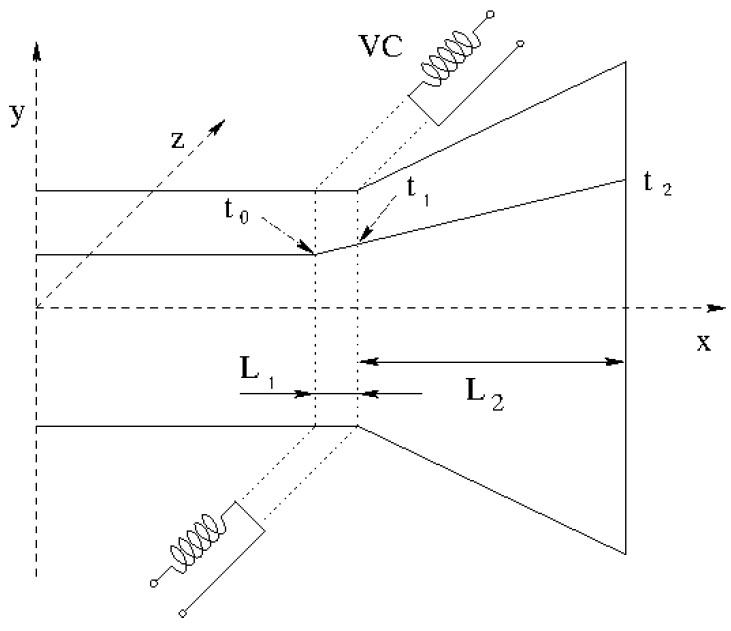
\includegraphics[scale=0.4]{scheme}
                \captionsetup{justification=centering, font=footnotesize}
                \captionof{figure}{Silové pusobení magnetického pole na elektronovy svazek. Elektrony vstupují do vychylovacího pole $B$ v case $t_0$ = 0 a servávají v ném po dobu $t_1$ na dráze $L_1$. Na dráze $L_2$ po dobu $t_2$ jiz nedocházi k vychylování. Lorentzova síla je nulová, dráha elektronu je prímková.}
                \label{fig:scheme}
                \vspace{10pt}
                \raggedright   

        \section{Měření}      
                \par Abyho bylo možné ověřit platnost vztahu (2), je třeba sestrojit graf závislosti $U_a$ = f($I^2_f$). Lineárním fitováním určíme směrnice $\alpha$ a vynásobením získané hodnoty konstantou $\frac{98r}{n^2}$ zjistíme ohniskovou vzdálenost čočky $f$. Výsledky jsou uvedeny na obrázku (2).
    \end{minipage}
\newpage
    \begin{minipage}[t]{0.5\textwidth} 
                \vspace{10pt}   
                \par \centering
                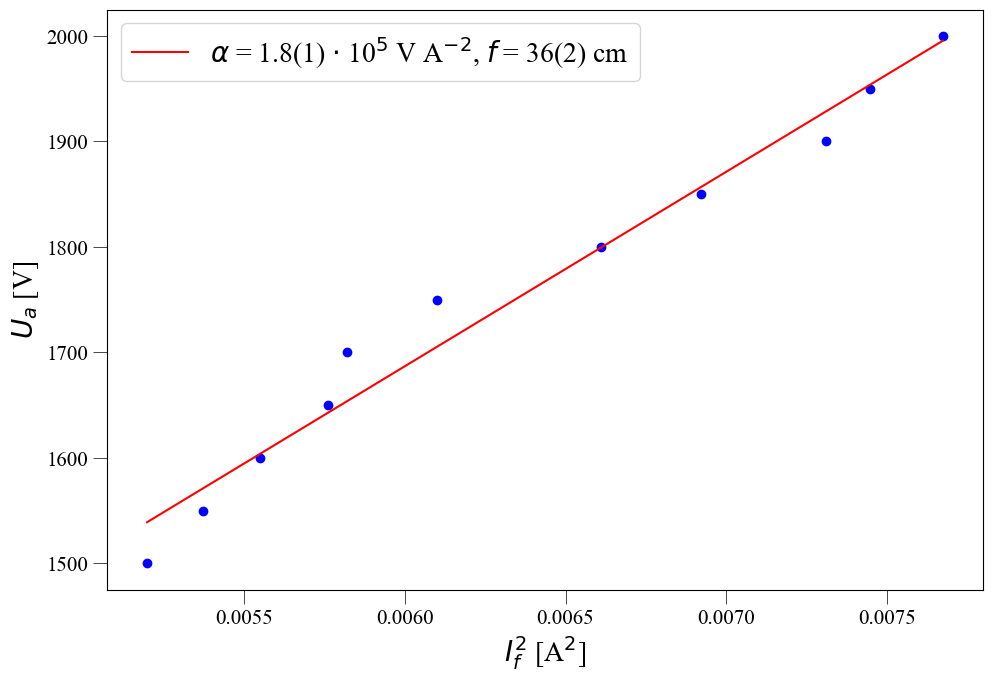
\includegraphics[scale=0.35]{ohn}
                \captionsetup{justification=centering, font=footnotesize}
                \captionof{figure}{Určení ohniskové vzdálenosti krátké magnetické čočky pomocí závislosti $U_a$ = f($I^2_f$).}
                \label{fig:ohn}
                \vspace{10pt}
                \raggedright  

                \par Odtud zjistíme hodnotu $f$: 
                \begin{center}
                    $f$ = 36(2) cm
                \end{center}

                \par Pro ověření platnosti vztahu (3) sestrojíme grafy závislosti výchylky $y$ a $Y$ na hodnotách $I_v$ a $U_a$ resp. Výsledky jsou uvedeny na obrázkech (3) a (4).

                \vspace{10pt}   
                \par \centering
                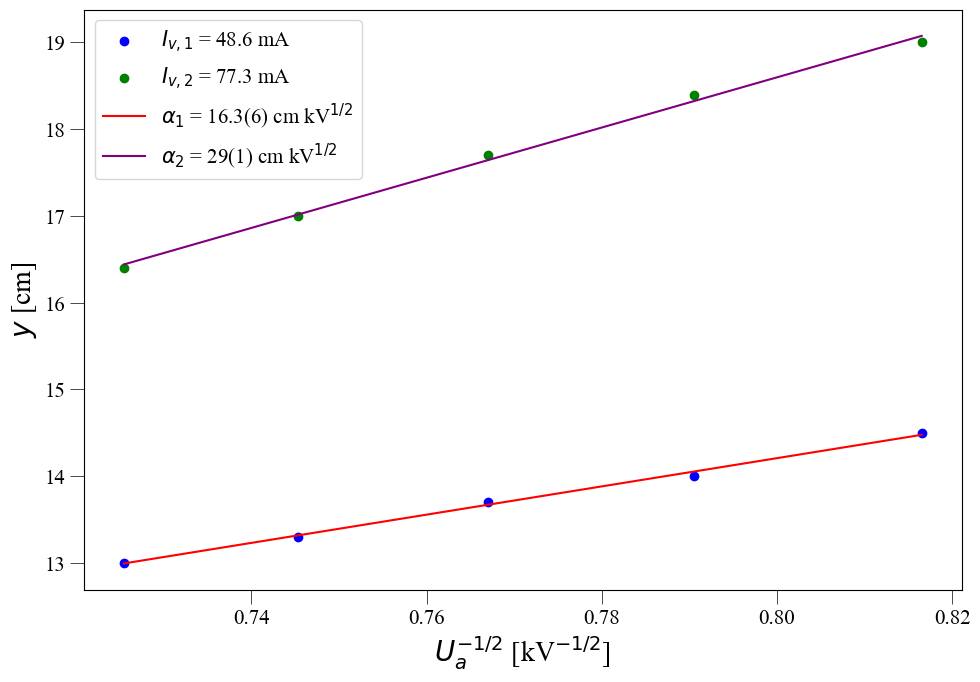
\includegraphics[scale=0.35]{u_v}
                \captionsetup{justification=centering, font=footnotesize}
                \captionof{figure}{Závislost výchylky $y$ na urychlovacím napětí $U_a^{-1/2}$.}
                \label{fig:u_v}
                \vspace{10pt}
                \raggedright  

                \vspace{10pt}   
                \par \centering
                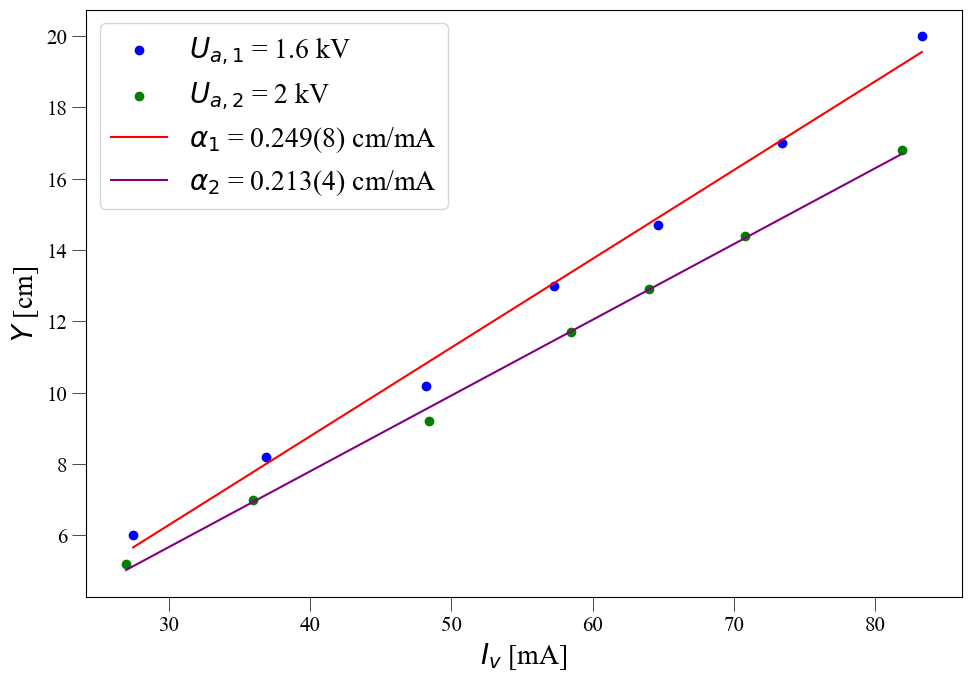
\includegraphics[scale=0.35]{I_v}
                \captionsetup{justification=centering, font=footnotesize}
                \captionof{figure}{Závislost výchylky $Y$ na vychylovacím proudu $I_v$.}
                \label{fig:I_v}
                \vspace{10pt}
                \raggedright  
    \end{minipage}
    \hspace{10pt}
    \begin{minipage}[t]{0.5\textwidth} 
                \par Při určování závislosti výchylky $y$ na urychlovacím napětí $U_a^{-1/2}$ jsme použili dvě hodnoty výchylkového proudu:
                \begin{center}
                    $I_{v,1}$ = 48.6 mA a $I_{v,2}$ = 77.3 mA
                \end{center}
                Z grafu je patrné, že získaná data skutečně odrážejí spravedlnost vztahu (3). To je patrné z linearity dat. Zejména je vidět, že sklon grafu pro větší hodnotu vychylovacího proudu je větší než pro menší hodnotu. 
                \begin{center}
                    $\alpha_1$ = 16.3(6) cm kV$^{1/2}$ < $\alpha_2$ = 29(1) cm kV$^{1/2}$
                \end{center}
                \par Při určování závislosti výchylky $Y$ na vychylovacím proudu $I_v$ jsme použili dvě hodnoty urychlovacího napětí:
                \begin{center}
                    $U_{a,1}$ = 1.6 kV a $U_{a,2}$ = 2 kV
                \end{center}
                Z grafu je patrné, že získaná data skutečně odrážejí spravedlnost vztahu (3). To je patrné z linearity dat. Zejména je vidět, že sklon grafu pro větší hodnotu urychlovacího napětí je menší než pro větší hodnotu.
                \par Tabulkové hodnoty použité při výpočtu:
                \begin{center}
                    $r$ = 2 cm a $n$ = 1000 
                \end{center}
                \par Výsledky měření jsou v tabulce (1).
                \vspace{10pt}
                \par K výpočtu veličin a jejich nejistot byla použita knihovna Uncertinties pro Python\cite{uncertainties}. Chyby byly rozšířeny o Studentův koeficient (2-Tail Confidence Level) s ohledem na stupně volnosti pro každou hodnotu, pro interval spolehlivosti 68.27\%.
        
        \section{Závěr} 
                Získaná hodnota ohniskové vzdálenosti krátké magnetické čočky $f$ = 36(2) cm pravděpodobně neodpovídá skutečnosti v plném smyslu. To je patrné z fyzických rozměrů zařízení, které jsou menší než získaná ohnisková vzdálenost. 
                \par Dále jsme potvrdili platnost vztahu (3). To jsme udělali pomocí sestrojení grafů závislosti výchylky $y$ a $Y$ na hodnotách $I_v$ a $U_a$ resp. Linearity dat a sklon grafů potvrzují spravedlnost vztahu (3).

                \renewcommand{\refname}{Odkazy}
                \begin{thebibliography}{9}
                    \bibitem{uncertainties}
                        Uncertainties, Dostupné online: \url{https://pypi.org/project/uncertainties}
                \end{thebibliography} 
    \end{minipage}
\newpage
    \begin{center}
        \section{Přílohy}
            \begin{center}
                \subsection{Tabulka naměřených hodnot} 
                    \pgfplotstabletypeset[
                        col sep=comma, % Defines the separator, comma for CSV
                        string type, % Treats columns as strings (not math mode)
                        every head row/.style={before row=\toprule,after row=\midrule},
                        every last row/.style={after row=\bottomrule},
                        columns/I_f/.style={column name=I_f [mA]},
                        columns/U_a/.style={column name=U_a [kV]},
                        columns/U_a_2/.style={column name=U_{a,1,2} [kV]^{[1]}, column type/.add={|}{}},
                        columns/y_1/.style={column name=y_1 [cm]^{[1]}},
                        columns/y_2/.style={column name=y_2 [cm]^{[1]}},
                        columns/I_v_1/.style={column name=I_{v,1} [mA]^{[2]}, column type/.add={|}{}},
                        columns/Y_1/.style={column name=Y_1 [cm]^{[2]}},
                        columns/I_v_2/.style={column name=I_{v,2} [mA]^{[2]}, column type/.add={|}{}},
                        columns/Y_2/.style={column name=Y_2 [cm]^{[2]}}
                    ]{data/data.csv}
            \end{center}

            \begin{enumerate}
                \item Hodnoty $y_1$ a $y_2$ byly změřeny pro hodnoty $I_{v,1}$ = 48.6 mA a $I_{v,2}$ = 77.3 mA resp. Pro oba meřené hodnoty napětí bylo stejné $U_{a,1,2}$.
                \item Hodnoty $Y_1$ a $Y_2$ byly změřeny pro hodnoty $U_{a,1}$ = 1.6 kV a $U_{a,2}$ = 2 kV resp.
            \end{enumerate}
\end{document}